\documentclass[a4paper, 12pt]{article}

\usepackage{graphicx}
\usepackage{caption}
\usepackage[section]{placeins}
\usepackage{fixltx2e}
\usepackage[page]{appendix}

\usepackage{amsmath}
\usepackage{cleveref}

%for code(MATLAB in particular)
\usepackage{listings}
\usepackage{color} %red, green, blue, yellow, cyan, magenta, black, white
\definecolor{mygreen}{RGB}{28,172,0} % color values Red, Green, Blue
\definecolor{mylilas}{RGB}{170,55,241}

% Default fixed font does not support bold face
\DeclareFixedFont{\ttb}{T1}{txtt}{bx}{n}{12} % for bold
\DeclareFixedFont{\ttm}{T1}{txtt}{m}{n}{12}  % for normal

% Custom colors
\usepackage{color}
\definecolor{deepblue}{rgb}{0,0,0.5}
\definecolor{deepred}{rgb}{0.6,0,0}
\definecolor{deepgreen}{rgb}{0,0.5,0}


\newcommand\pythonstyle{\lstset{
language=Python,
basicstyle=\ttm,
otherkeywords={self},             % Add keywords here
keywordstyle=\ttb\color{deepblue},
emph={MyClass,__init__},          % Custom highlighting
emphstyle=\ttb\color{deepred},    % Custom highlighting style
stringstyle=\color{deepgreen},
frame=tb,                         % Any extra options here
showstringspaces=false            % 
}}

\lstnewenvironment{python}[1][]
{
\pythonstyle
\lstset{#1}
}
{}

\newcommand\pythonexternal[2][]{{
\pythonstyle
\lstinputlisting[#1]{#2}}}


\lstset{
    language=Matlab,%
    %basicstyle=\color{red},
    breaklines=true,%
    morekeywords={matlab2tikz},
    keywordstyle=\color{blue},%
    morekeywords=[2]{1}, keywordstyle=[2]{\color{black}},
    identifierstyle=\color{black},%
    stringstyle=\color{mylilas},
    commentstyle=\color{mygreen},%
    showstringspaces=false,%without this there will be a symbol in the places where there is a space
    numbers=left,%
    numberstyle={\tiny \color{black}},% size of the numbers
    numbersep=9pt, % this defines how far the numbers are from the text
    emph=[1]{for,end,break},emphstyle=[1]\color{red}, %some words to emphasise
    %emph=[2]{word1,word2}, emphstyle=[2]{style},
}


\graphicspath{{./pictures/}}

\title{ECEN321 - Lab 2 \\
    Noise
}
\author{Joshua Benfell - 300433229}

\begin{document}
	\maketitle
    
    \section{Introduction}

        This report investigates noise and how it propagates through operations and ways at reducing the effect noise has on systems. To do this various applications where noise would be present will be simulated.

    \section{Applications}
        \subsection{Amplifier}
            The first application being simulated is a voltage amplifier. This amplifier will have a voltage gain of $10$ and a normally distributed signal of DC level $3V$ with variance $4 V^2$ will be put through it.
            \par
            The method of signal averaging will be applied to the original signal. For this 16 signals generated the same way will be averaged. Increasing the number of samples will decrease the standard deviation by $\sigma = \frac{\sigma}{\sqrt{N}}$, so by using 16 signals we expect an an approximate reduction of $\frac{1}{4}$. 
        \subsection{AC Signal}
            Another application where noise is prevalent is alternating current. This can be represented for a low amplitude sinusoid with an amplitude of $1V$. For this application a large amount of noise with $\sigma^2 = 1$ will be applied as there are cases where the original signal is indistinguishable from what is desired. To compare how closely related these signals are, the covariance and correlation coefficients will be used.
        \subsection{Voltmeters}
            Voltmeters are commonly used measuring devices which, like all measuring devices have some uncertainty in their measurements. This is amplified when multiple signals are involved before a measurement has taken place. For this simulation two signals will be used which take the form $V_1 = 1.934 \pm 0.001$ and $V_2 = 2.53 \pm 0.01$; both signals are uniformly distributed. The resulting signal of $V_2 - V_1$ will be ``measured'', and the resulting PDF will be plotted.

        
    \section{Results and Discussion}
        \subsection{Amplifier}
            \begin{figure}[!t]
                \centering
                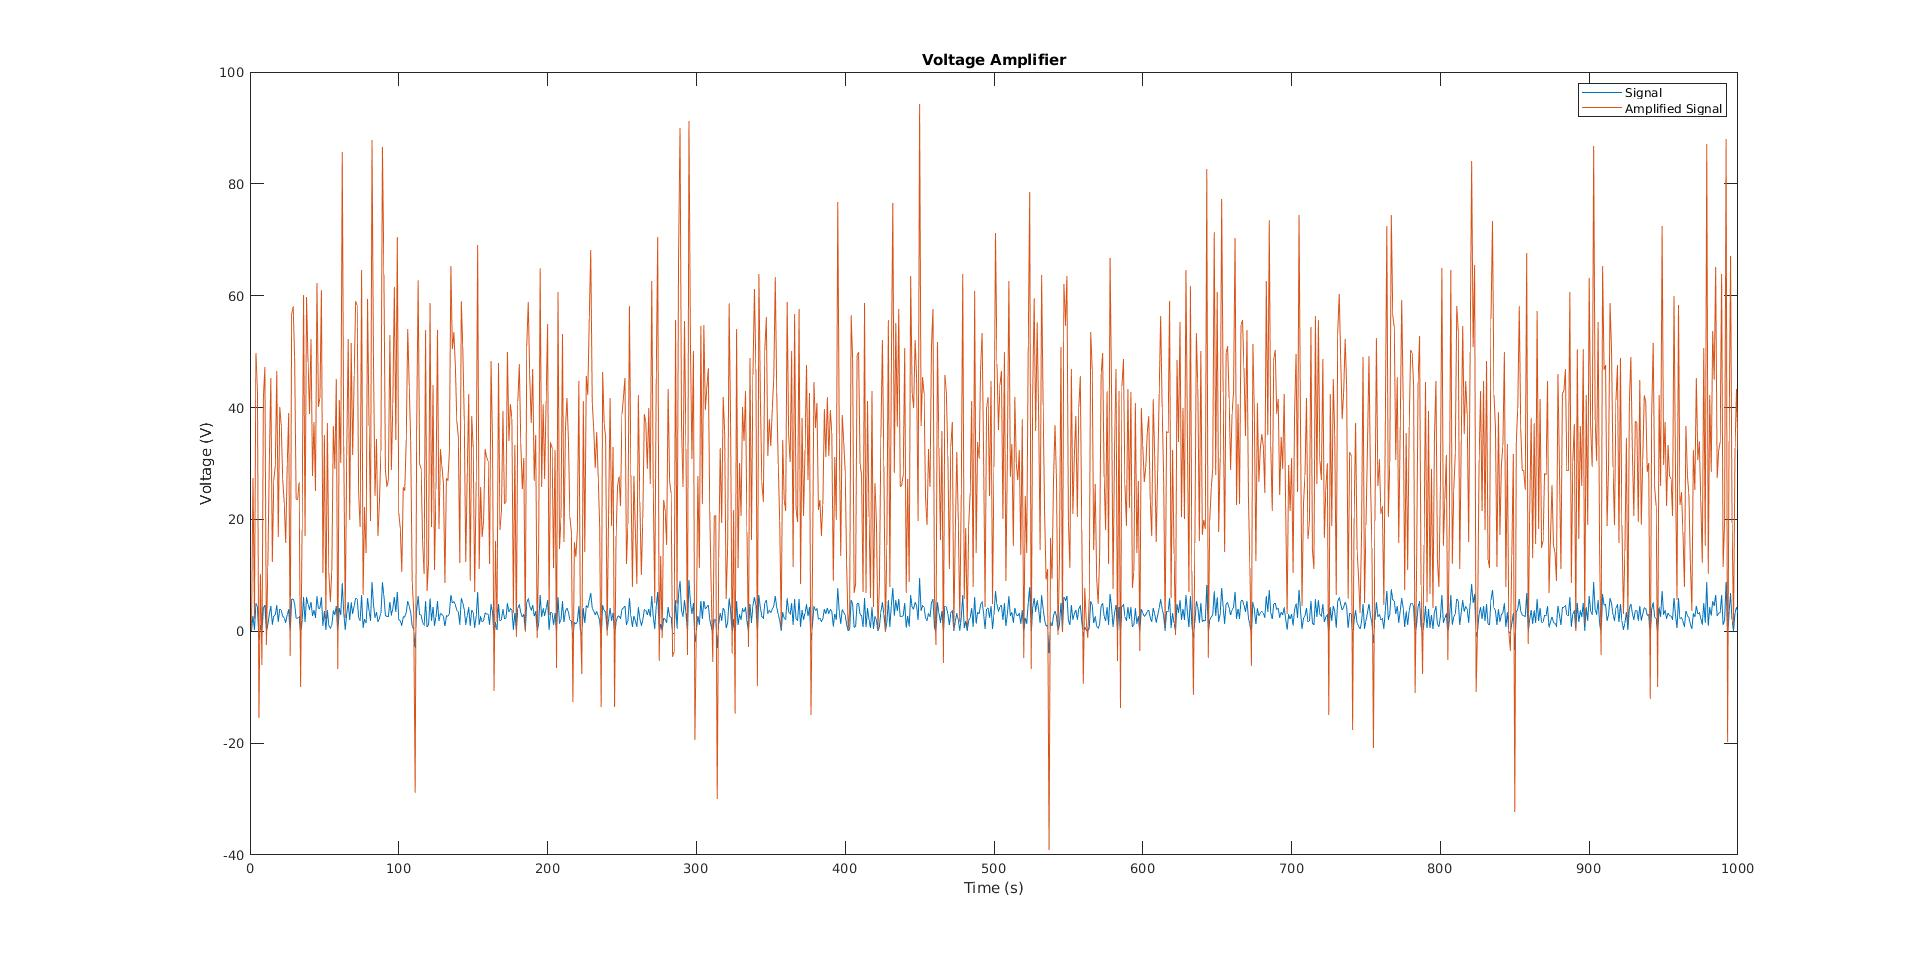
\includegraphics[width=\textwidth]{amplifier.jpg}
                \caption{Voltage signals before and after amplification}
                \label{fig:amp}
            \end{figure}

            \begin{figure}[!t]
                \centering
                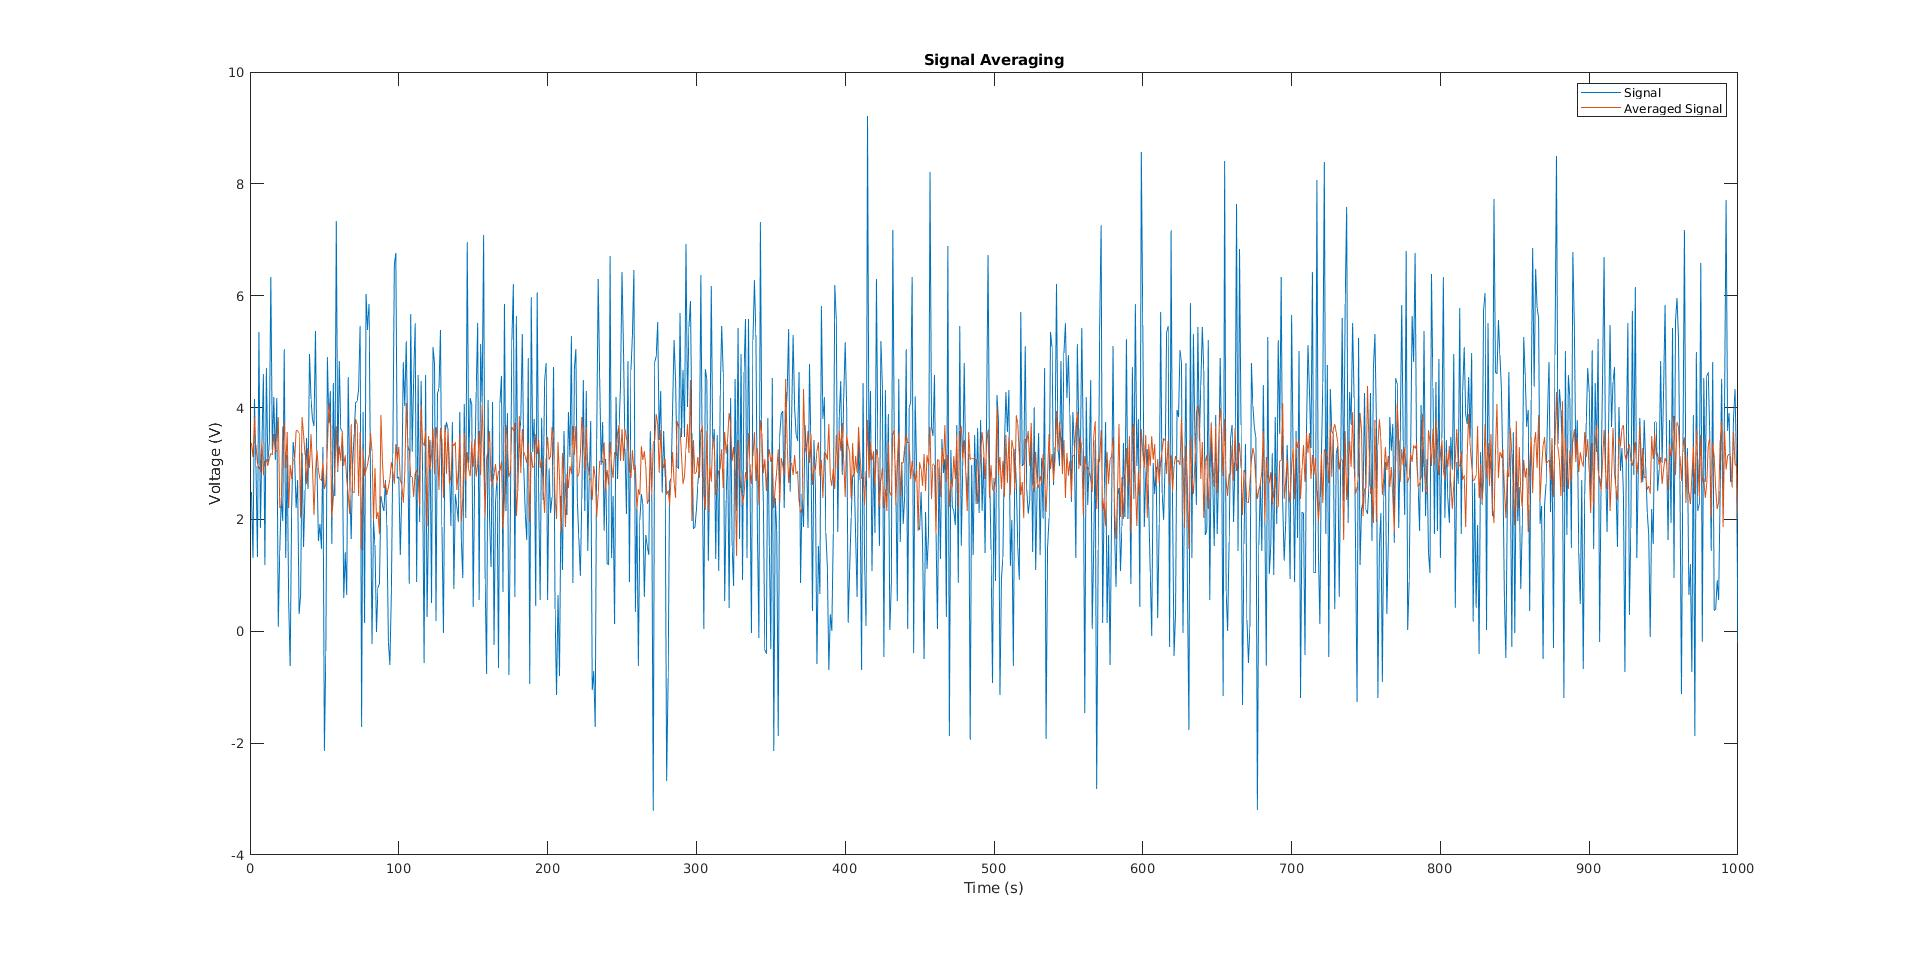
\includegraphics[width=\textwidth]{averaging.jpg}
                \caption{Voltage signals before and after averaging}
                \label{fig:ave}
            \end{figure}

            The original signal had $\mu = 3.0418$ and $\sigma = 2.0041$. These values are fairly close to the set values of 3 and 2, and the signal can be seen in \cref{fig:amp}. After amplifying this signal the follownig values were recorded: $\mu = 30.4184$ and $\sigma = 20.0405$. From this we can see that when a signal with uncertainty is multiplied by a constant both terms are multiplied. This has major implications on signal with noise as we now have a massive deviation from the target $30V$, even to the point where it's very negative. This is visible in \cref{fig:amp}, and is not ideal for practical use.
            \par
            As the above results are non-ideal, the noise should be reduced. As mentioned above, a method of doing so is to average many signals. A difference between the averaged signal and the original signals should be visible from viewing the mean and standard deviation of one of the used signals. One of these signals values is $\mu = 2.9038$ and $\sigma = 1.9926$. After averaging the new values are $\mu = 2.9809$ and $\sigma = 0.5017$. From this and \cref{fig:ave} we can see that the standard deviation ($\sigma$) has decreased by approximately a factor of 4 as hypothesized and that the mean has gotten closer to the true value. The change to the mean is likely from the removal of extreme values that were introduced by the larger noise. This emphasizes the importance of taking many measurements as precision is increased, and in extreme cases like this, the accuracy may be improved (or you'll get a better idea of the bias).

        \subsection{AC Signal}
            \begin{figure}[!t]
                \centering
                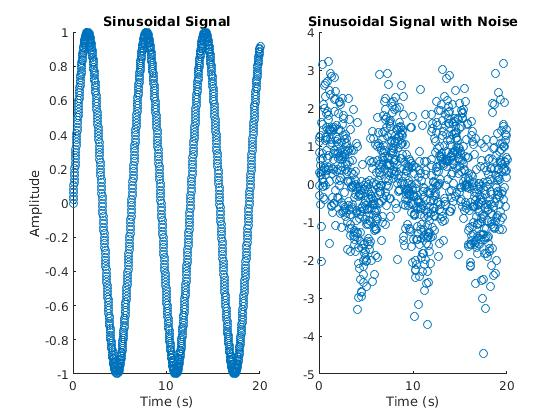
\includegraphics[width=\textwidth]{sine.jpg}
                \caption{Sinusoidal signals before and after adding noise}
                \label{fig:sin}
            \end{figure}
            \begin{figure}[!t]
                \centering
                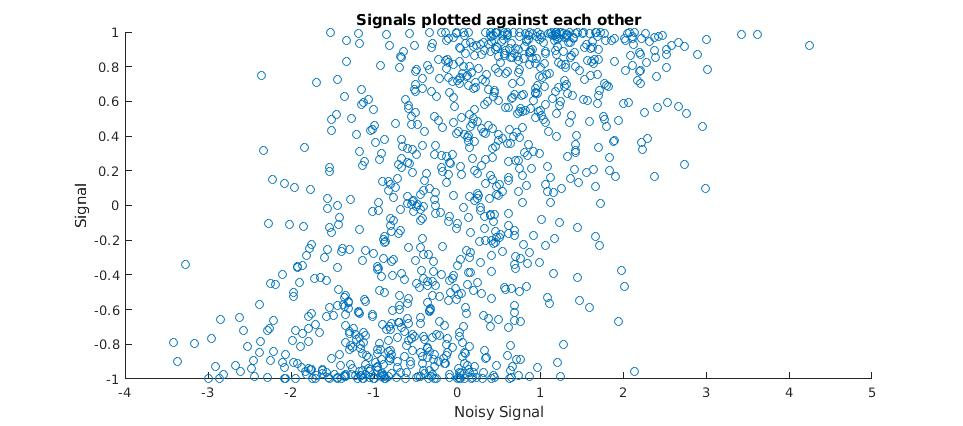
\includegraphics[width=\textwidth]{signals.jpg}
                \caption{Sinusoidal signals with and without noise plotted against each other}
                \label{fig:sigs}
            \end{figure}

            \[Cov = 
            \begin{bmatrix}
                0.4902  &  0.4828 \\
                0.4828  &  1.4863
                \label{mat:cov}
            \end{bmatrix}\]
            
            After applying the noise to the sinusoid it can be seen in \cref{fig:sin} that the sinusoid is faintly visile in the scatter plot. The peaks and troughs are much lower and higher than expected though in some places. For comparing how closely related the new and old values are, the covariance and correlation coefficient are taken. The covariance matrix for the two datasets is above, the important value being the off diagonal (these are the same value), which is the covariance between the two sets. This value is 0.4828, which is positive indicating a positive relationship, is also small, indicating that the relationship is not strongly correlated. This indicates the noise on a signal can greatly distort it from being visible as the original signal. Because the time scale is tighter, it is possible to see the sinusoidal shape, but due to the large spread around the darker areas it is possible to understand how this can not be seen as a sinusoid anymore, or close to. 
            \par
            The other variable gathered is the correlation coefficient which for this run of the program was $\rho = 0.5656$. This indicates that there is a moderate positive relationship \cite{rumsey_2020}, which can be seen when plotted against each other in \cref{fig:sigs}. Some correlation can be seen but there is lots of noise which make some of the data look essentially like noise. 

        \subsection{Voltmeters}
            \begin{figure}[!t]
                \centering
                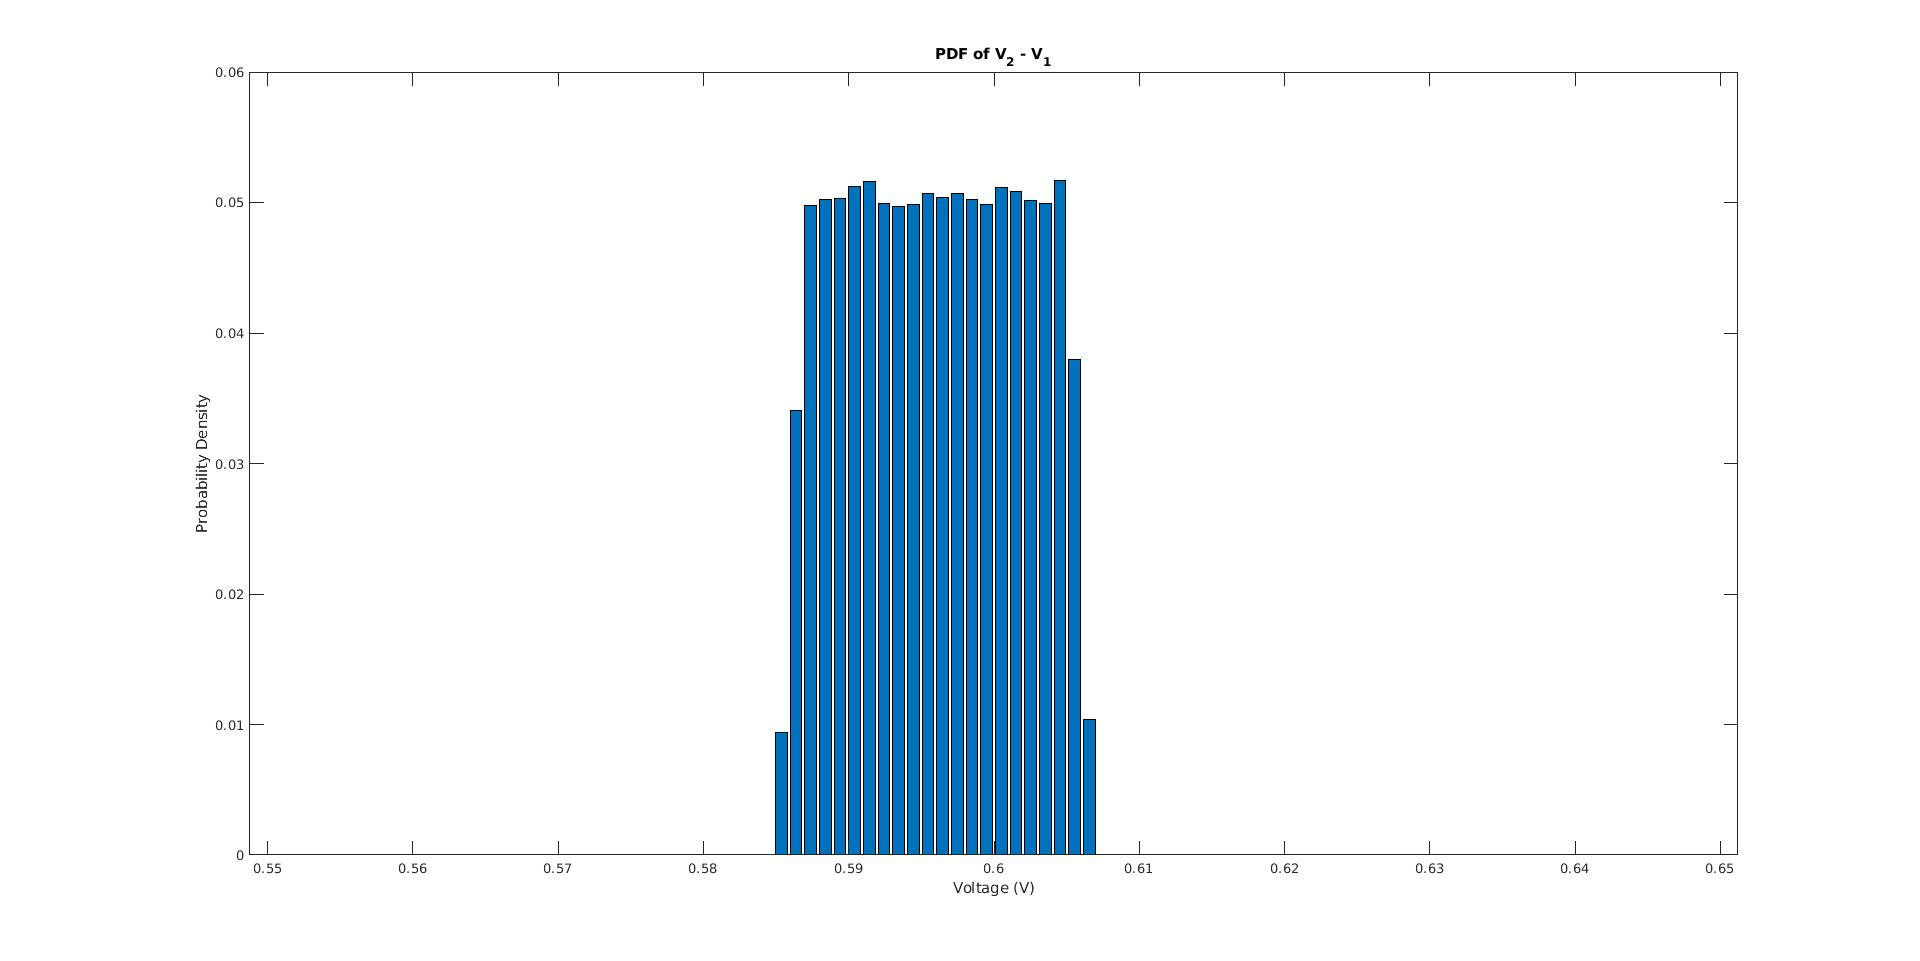
\includegraphics[width=\textwidth]{V3.jpg}
                \caption{PDF of $V_2 - V_1$}
                \label{fig:v3}
            \end{figure}
            
            The final application explores the effect of two signals with noise being measured after one is subtracted from the other. By using two uniformly distributed signals we can see in \cref{fig:v3} that we get a uniformly distributed signal as a result. This signal has mean $\mu = 0.5960$ and std dev $\sigma = 0.0058$, and these values are consistent over multiple simulations. The mean is exactly the answer to $2.53-1.934$ and the standard deviation is close to the mean of the uncertainties, although this is less significant as the uncertainty is not the standard deviation. The final standard deviation is equal to the standard deviation of $V_2$ as the standard deviation of $V_1$ is on the order of $10^{-4}$ which matlab removes through rounding so we don't see it's effect initially. Multiplying by 1000 reveals that it's $0.0058051$ which is the sum of the standard deviviations of both $V_1$ and $V_2$. 


    \section{Conclusion}
        The main take aways from this report are that, repeated measurements reduce the standard deviation by a facter of $\sqrt{N}$, increasing precision. This is important as any constant that multiplies a measurement with some uncertainty also multiplies the uncertainty, making it larger.
        \par
        The addition of noise to a signal can make that signal much less distinguishable in shape from what it is. This only happens if the size of the noise is a significant percentage (including higher) than the amplitude of the wave as instead of following the signals shape it extends far past it.
    % \Urlmuskip=0mu plus 1mu\relax
    \bibliography{bibliography}
    \bibliographystyle{IEEEtran}

    \begin{appendices}
        \section{Q1 Code}
            \lstinputlisting{../q1.m}
        \section{Q2 Code}
            \lstinputlisting{../q2.m}
        \section{Q3 Code}
            \lstinputlisting{../q3.m}
        \section{Q4 Code}
            \lstinputlisting{../q4.m}
    \end{appendices}
\end{document}